\section{Data Center vs. WAN Latency}

\subsection{Methodology}
Our primary goal in this section is to understand the percentage of total round-trip time (as experienced by end-users) spent inside of the data center (DC). We designed the following experiment to perform queries to data centers. We present the model of communication we expect between end-users and the DC in Fig.\,\ref{fig:DC_model}, as well as the latency measurements we will collect. 

\begin{figure}
  \centering
  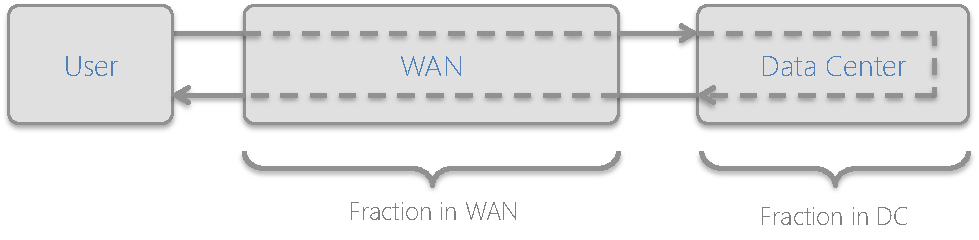
\includegraphics[width=\linewidth]{../figs/DC_model.pdf}
  \caption{Typical User-DC communication pattern}
  \label{fig:DC_model}
\end{figure}

We have chosen Google Search as a representative user-facing service for our case study. One reason for choosing Google Search is that the service provides a metric of estimated time spent within the DC (Fig.\,\ref{fig:google_time}). From our analysis in Sec.\,\ref{sec:analysis}, we believe this data to be fairly accurate in reflecting the fraction of round-trip time spent inside the DC.

\begin{figure}[t]
  \centering
  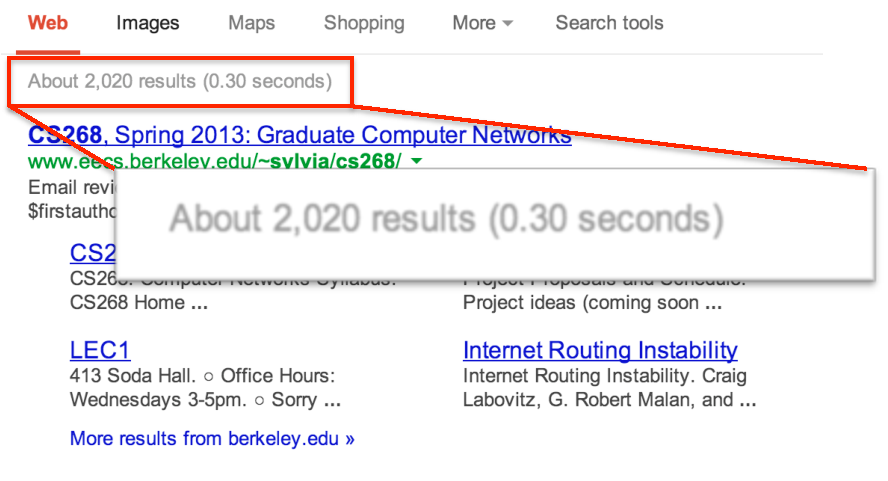
\includegraphics[width=0.85\linewidth]{../figs/GoogleTime.pdf}
  \caption{Google Search estimated time spent within DC as presented in the search results page}
  \label{fig:google_time}
\end{figure}

We perform a query at the end-host and time-stamp the start and end times. In this way we can measure the complete round-trip time for a single query as experienced by the end-host. The largest hurdle is selecting a search term to query. Initially, we suspected that caching within the DC would impact our results. Thus, we believed that "hot trends" (Google's own reported highest searched terms) were likely to be cached. As such, they would provide a baseline measurement for understanding the WAN latency as minimal time spent would be spent within the DC. On the other hand, we use a random string in our  queries minimize the probability of caching and force the query to be processed. We extracted "hot trends" from Google Trends\footnote{http://www.google.com/trends/hottrends}, and we generate random strings of length 32, comprised of numbers and letters (both lower and uppercase). Our analysis in Sec.\,\ref{sec:analysis} shows that the results of our measurements produced differed greatly from our original assumptions. Nonetheless, we believe this methodology is useful in understanding the fraction of round-trip time spent inside the DC.

To provide context for our measurements, we perform {\it ICMP ping} queries to measure the network latency from the end-user to Google. Because we conduct this experiment in a geographically distributed fashion and because Google has many user-facing servers/IPs, we must take additional steps to ensure the server being pinged is in fact responsible for handing our search queries. We process the application layer HTTP conversation at the using {\it tcpdump} to capture all the packets and extract the IP of the Google server.
 
In Table \ref{tab:DC_method} we provide an overview of the four different ``time'' measurements derived from our experiment.

\begin{table}
  \begin{tabular}{p{2.8cm} | p{5cm}}
    \hline
    type & description \\
    \hline
    Hot-trend-query time & the time spent to query a hot trend word to Google. \\
    Random-query time & the time spent to query a 32-character random string.  \\
    Ping time & the networking layer round-trip time to the responded Google IP address. \\
    Google time & Google's own estimated time spent within their DC. \\
    \hline
  \end{tabular}
  \caption{Four different ``times'' measured}
  \label{tab:DC_method}
\end{table}


% \begin{itemize}
% \setlength{\leftmargin}{-1pt}
% \setlength{\itemsep}{1pt}
% \setlength{\parskip}{0pt}
% \setlength{\parsep}{0pt}
% \item Hot-trend-query time \\
%   the time spent to query a hot trend word to Google. 
% \item Random-query time -- the time spent to query a 32-character random string. 
% \item Ping time -- the networking layer round-trip time to the responded Google IP address.
% \item Google time -- Google's estimated time spent within their DC.
% \end{itemize}


\subsection{Implementation and Experiment}
\label{sec:impl-exper}


We implemented our measurement script in Python, and use {\it cron} to schedule the execution every two hours. In each pass, the script will first visit Google Trends webpage and obtain the hot-trend words for that hour. Along with randomly generated strings, we create a list of 20 strings to query. 
The entire list is queried repeatedly 10 times, and the four ``times'' are recorded. Each query is conducted using Python urllib2 library over HTTP, using the query address \url{http://www.google.com/search?hl=en\&output=search\&q=query}.\footnote{One thing to note about our implementation is that it violates Google's terms of service, as sending automated queries is disallowed. In the event automated queries are detected, Google responds with a page containing the following message: ``Our systems have detected unusual traffic from your computer network.'', and the users will be required to enter a CAPTCHA. The workaround we utilize is to limit the query speed. So after each query, we delay the script for 5 seconds. We should point out that there are at most $12\times20$ queries per day, which limits our sample size.}

While performing a query, we utilize {\it tcpdump} to monitor the incoming and outgoing traffic on port 80. By inspecting the TCP traces, we can find the specific Google IP that responds our query. We then {\it ping} this IP 10 times and record the results. {\it tcpdump} and {\it ping} are invoked using Python subprocess module.

\subsection{Analysis}
\label{sec:analysis}

Present the results and describe what we learned from the data.
Consider putting an appendix of all Planet Lab nodes we have used.

\begin{figure*}[!htb]
  \centering
  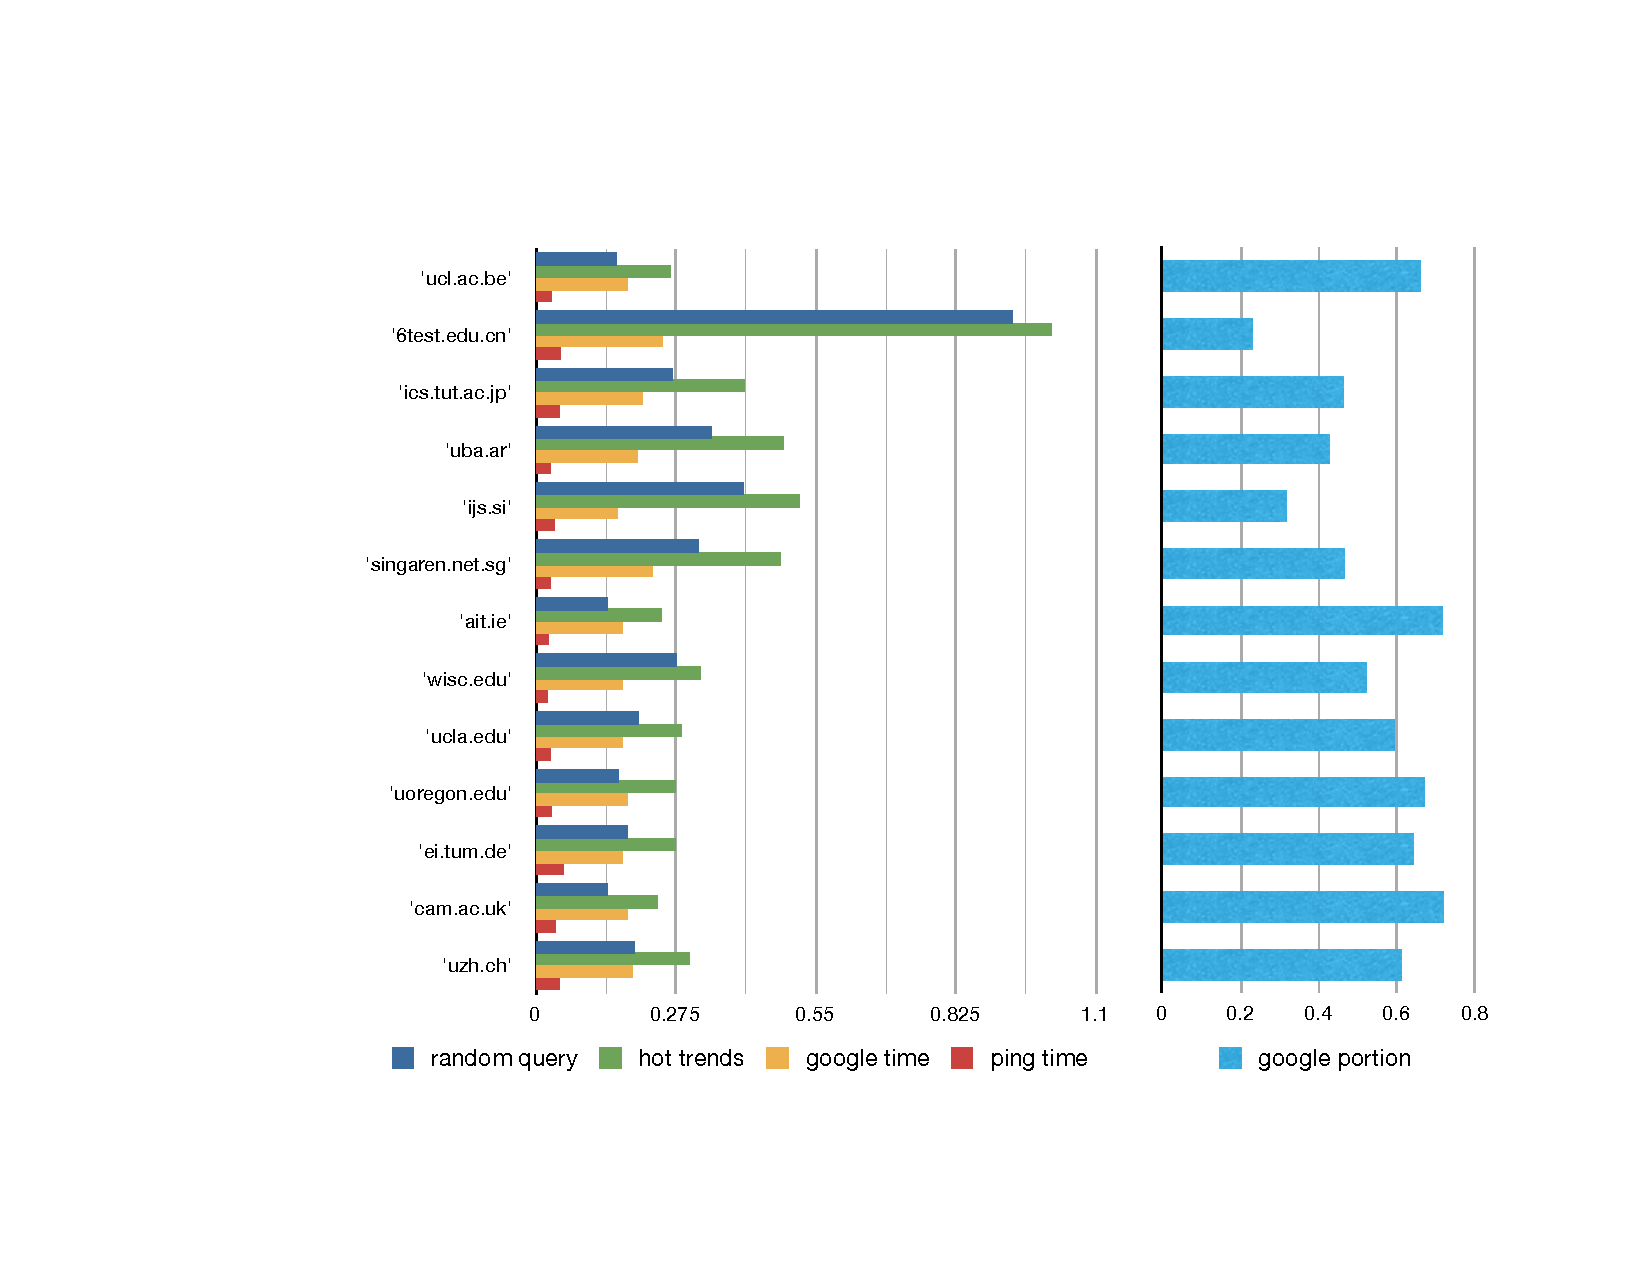
\includegraphics[width=\linewidth]{../figs/data_center.pdf}
  \caption{The latency measured in DC conversation experiments}
  \label{fig:data_center}
\end{figure*}


%%% Local Variables: 
%%% mode: latex
%%% TeX-master: "main"
%%% End: 

